\documentclass[11pt,a4paper]{scrartcl}
\typearea{12}
\usepackage{graphicx}
\usepackage{pstricks}
\usepackage{listings}

\usepackage{tikz}

\usepackage{pgf}
\usepackage[utf8]{inputenc}
\usetikzlibrary{arrows,automata}
\usetikzlibrary{positioning}


\tikzset{
    neuron/.style={
           rectangle,
           rounded corners,
           draw=black, very thick,
           inner sep=2pt,
           text centered,
           },
}


\tikzset{
    gc/.style={
           rectangle,
           rounded corners,
           draw=red, very thick,
           inner sep=2pt,
           text centered,
           },
}


\tikzset{
    io/.style={
           rectangle,
           rounded corners,
           draw=green, very thick,
           inner sep=2pt,
           text centered,
           },
}



\lstset{language=python}
\pagestyle{headings}
\markright{Computational Neuroscience - 12 conditioning}
\begin{document}


\begin{figure}
\begin{center}
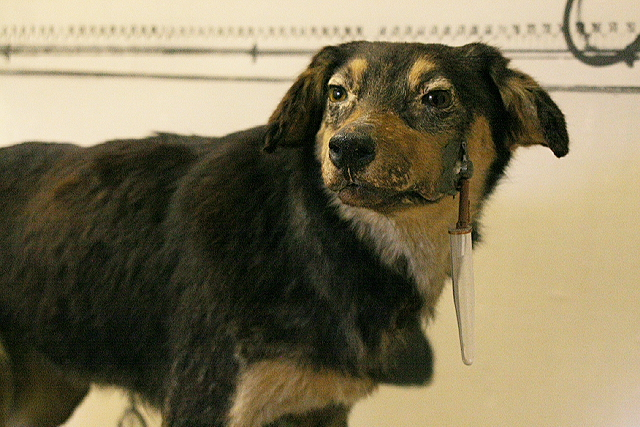
\includegraphics[width=7cm]{One_of_Pavlovs_dogs.jpg}%
\end{center}
\caption{This is a picture of one of Pavlov's dogs, it has been stuffed and is preserved at The Pavlov Museum. You can see where the salvia tube and container has been implanted. [Picture from \texttt{http://en.wikipedia.org/wiki/Ivan\_Pavlov}]}
\end{figure}


\subsection*{Introduction}
These notes are about the classical conditioning and the mesocortical
dopaminergic pathway which is believed to be responsible for the
brain's \textsl{reward system}. 

\subsection*{Classical conditioning}

\begin{quote}
Pavlov is the biggest fool I know; any policeman could tell you that much
about a dog. - George Bernard Shaw
\end{quote}

In Pavlov's famous experiment, conduction at the turn of the
nineteenth and twentieth centuries, a bell is rung a short time before
a dog is fed; obviously feeding causes salivation in the dog, but the
curious thing is that after a while the dog salivates as soon as it
hears the bell. This experimental and the conclusion that were drawn
from it were hugely controversial at the time, opinions ranged from
Shaw's above, claiming that nothing interesting had been measured or
concluded.  For its proponents, Pavlovian conditioning seemed to
promise a new scientific era of psychology and even promised the
\lq{}the perfectibility of man\rq{} and featured, for example, in
Aldous Huxley's dystopian novel \textsl{Brave New World} and his
utopian novel \textsl{The Island}. As for Shaw:
\begin{quote}
If ‘A’ is drowning on one side of a pier and ‘B’ is equally drowning on the
other, and you have one lifebelt, to which of the two would you like to throw
it? Which would I save, Pavloff or Shaw? What is the good of Shaw? And
what is the good of Pavloff? Pavloff is a star which lights the world, shining
above a vista hitherto unexplored. Why should I hesitate with my lifebelt for
one moment? - H.G. Wells
\end{quote}

These days we describe the bell as an \textsl{conditioned stimulus}
(CS), it produces salivation only after training, the food is an
\textsl{unconditioned stimulus} (US), it always produces response. In
other words, the US is the food since it already produces the
reaction: salivation, whereas the bell is the CS since it only
produces the response after training, that is, after
conditioning. Classical, or Pavlovian, conditioning is also
distinguished from \textsl{instrumental} or \textsl{operant}
conditioning in which the actions of animal determine the
reinforcement; like Pavlovian conditioning, operant conditioning has a
controversial history, it is associated with another behaviourist,
B.F. Skinner, but away from the complex philosophical and political
interpretations, both forms of conditioning are now important
neuroscientific tools.

\subsection*{Models of classical conditioning}

The widely used Rescorla-Wagner model of classical conditioning works
\cite{RescorlaWagner1972a} like a perceptron; based on the stimulus
the animal anticipates a reward and adjusts its prediction according
to its accuracy. Hence, if $x$ is a binary value representing the
presence or absence of the stimulus, $r>0$ is the reward; a negative
$r$ would correspond to an aversive event, $v$ is the predicted reward and $w$ the weight used by the animal to predict the reward:
\begin{equation}
v=wx
\end{equation}
The Rescorla-Wagner rule is then
\begin{equation}
w\rightarrow w+\eta \delta x
\end{equation}
where $\delta =r-v$ is the error in prediction and $\eta$ is a
learning rate. These dynamics are illustrated in \ref{fig:w}.

\begin{figure}
\begin{center}
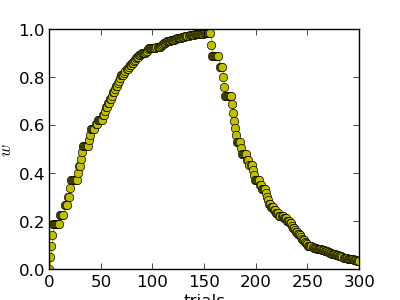
\includegraphics{RW.png}%
\end{center}
\caption{Changes in $w$. In each trial a stimulus is presented with probability 0.5; during the first 150 trials the stimulus is accompanied by a reward of $r=1$, after that by $r=0$. Plotted is the resulting Rescorla-Wagner changes in $w$ as it learns the reward and as the conditioning is extinguished. The learning rate is $\eta=0.05$. This is roughly based on a similar figure in \cite{DayanAbbott2001a}. \label{fig:w}}
\end{figure}

The Rescorla-Wagner rule generalizes to more than one stimulus-reward pair. Say $x_i$ is the binary value representing the presence or absence of the $i$th stimulus and $r_i$ is the corresponding reward, then the total reward is
\begin{equation}
r=\sum_i x_ir_i
\end{equation}
and the predicted reward is
\begin{equation}
v=\sum_i x_iw_i
\end{equation}
and the learning rule is
\begin{equation}
w_i\rightarrow w_i+\eta\delta x_i
\end{equation}
where $\delta=r-v$ as before. 

One significant victory for this proposal is that it explains
blocking. Consider conditioning a reward $r$ on a stimulus $s_1$ and
then changing so that there are two stimuli used to predict $r$, $s_1$
and $s_2$; now, when $s_2$ is shown on its own to the animal it does
not anticipate the reward. Thus, for example, Pavlov's dog might be
shown a light just before it is fed and will soon salivate when it
sees the light; next a light is lit and a bell rung before feeding,
now, if the bell is rung on its own, the dog does not salivate; the
light has \textsl{blocked} the bell. This is an easy consequence of
the Rescorla-Wagner rule since the $w$ for the light already gives a
correct prediction of the target and so the $w$ for the bell stays at
zero as there is no error. Blocking is not a consequence of other
models of conditioning proposed at the same time. It has, however,
been observed in behavior.
\cite{MillerEtAl1995a,AzorlosaCicala1986a}.

\subsection*{Ventral tegmental area}

The ventral tegmental area (VTA) is located immediately beside the
substantia nigra (SN) in the midbrain. In Wikipedia it says \lq{}[VTA] is
important in cognition, motivation, orgasm, drug addiction, intense
emotions relating to love, and several psychiatric disorders.\rq{} We
are interested in it here because it is believed to play an important
role in the reward system. 

The VTA has a large number of dopaminergic neurons, dopamine is a
neuromodulator; the level of dopamine alters the dynamics of synapses:
different synapses have different dopamine receptors and so their
dynamics might be altered in different ways. Dopaminergic neurons are
not common, there are about 400,000 in the human brain, about half of
these are in the VTA and half of VTA neurons are dopaminergic. these
dopaminergic neurons project to diverse areas in the brain, see
Fig.~\ref{fig:VTA}, including hippocampus, basal ganglia and the
prefrontal cortex. These projections transmit dopamine to these
areas. Another peculiarity of VTA is that contains a large number of
gap junctions.

\begin{figure}
\begin{center}
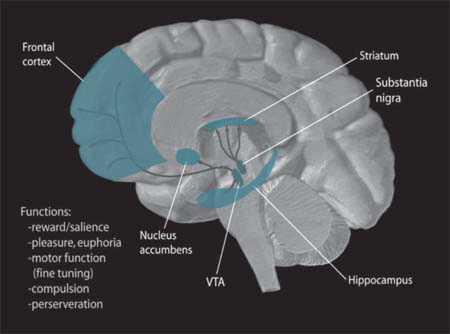
\includegraphics[width=7cm]{Dopamine_Pathways.png}
\end{center}
\caption{This shows the dopamine pathways from VTA and from SN; VTA
  has major projections to hippocampus, the nucleus accumbens in the
  basal ganlia and to the prefrontal cortex. [Picture from
    \texttt{http://en.wikipedia.org/wiki/Dopamine}]\label{fig:VTA}}
\end{figure}

The idea here is that $\delta$, the error, is calculated in
dopaminergic VTA neurons and that neuromodulation produces the
Rescorla-Wagner rule. This is sketched out in
Fig.~\ref{fig:circuit}. Evidence for this can be seen in a famous
experiment \cite{SchultzDayanMontague1997a} in which the activity of
dopaminergic cells was recorded in monkeys during conditioning. Before
condition the dopaminergic neurons fire at an elevated rate when the
reward is received, after conditioning they fire at a depressed rate
if the anticipated reward fails to appear after the stimulus, Fig.~\ref{fig:spikes}.

\begin{figure}
\begin{center}
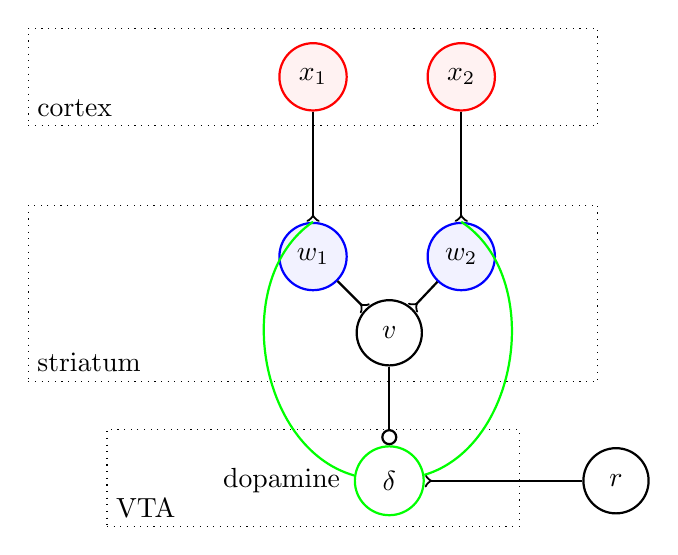
\begin{tikzpicture}
\node[text width=7cm, text height=1cm, draw=black, dotted](SC){cortex};
\node[align=center,text width=0.5cm,circle,draw=red, thick, fill=red!5](x1){$x_1$}; 
\node[align=center,text width=0.5cm,circle,draw=red, thick, fill=red!5, right = 1cm of x1](x2){$x_2$};
\node[text width=7cm, text height=2cm, draw=black, dotted,below =1cm of SC](St){striatum}; 
\node[align=center,text width=0.5cm,circle,draw=blue, thick, fill=blue!5,below = 1.4cm of x1](w1){$w_1$}; 
\node[align=center,text width=0.5cm,circle,draw=blue, thick, fill=blue!5, right = 1cm of w1](w2){$w_2$};
\node[align=center,text width=0.5cm,circle,draw=black, thick, below right= 0.5cm of w1](v){$v$};
\path (x1) edge[thick,-<] (w1);
\path (x2) edge[thick,-<] (w2);
\path (w1) edge[thick,-<] (v);
\path (w2) edge[thick,-<] (v);
\node[text width=5cm, text height=1cm, draw=black, dotted,below =0.6cm of St](VTA){VTA}; 
\node[align=center,text width=0.5cm,circle,draw=green, thick, below = 1cm of v](delta){$\delta$};
\node[left = 0.05cm of delta](d){dopamine};
\path (v) edge[thick,-o] (delta);
\node[align=center,text width=0.5cm,circle,draw=black, thick, right= 2cm of delta](r){$r$};
\path (r) edge[thick,-<] (delta);
\path (delta) edge[thick,green,bend left =  65] (w1.north);
\path (delta) edge[thick,green,bend right = 65] (w2.north);
\end{tikzpicture}
\end{center}
\caption{A schematic of the VTA reward circuit. The conditioned
  stimulus is presented and this is communicated via the cortex,
  neurons in the striatum adjust this to give the input $w_ix_i$ and
  these are added producing the estimated reward. This inhibits a
  dopaminergic neuron in VTA, this neuron also receives excitatory
  input corresponding to the actual reward, this difference is
  $\delta$ and $\delta$ is effects dopamine modulation $w_1$ and $w_2$
  effecting some version of the  Rescorla-Wagner rule.\label{fig:circuit}}
\end{figure}

\begin{figure}
\begin{center}
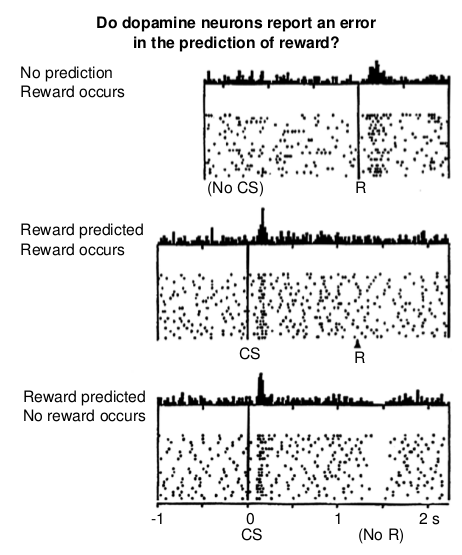
\includegraphics[width=7cm]{Schultz.png}
\end{center}
\caption{Dopaminergic cell activity. In the top panel there has been
  no conditioning, this means the predicted reward is zero and the
  dopaminergic neurons firing corresponding to a positive error; the
  reward exceeded expectation. The bottom panel shows what happens
  after conditioning if the reward is not received, since a reward is
  predicted this is a negative error and depresses firing. The middle
  panel shows that the consequence of conditioning is to advance the
  dopamine firing forward in time. [Figure taken from \cite{SchultzDayanMontague1997a}]. \label{fig:spikes}}
\end{figure}

Another thing is apparent from Fig.~\ref{fig:spikes}: when the animal
has been conditioned the dopaminergic neurons fire at the stimulus,
the activity shifts forward from reward to the stimulus that predicts
it. In a way this makes sense, the unanticipated event is the
stimulus; this predicts the reward but is itself a surprise. This is
also obviously useful, it allows the credit for the reward to be
usefully associated with the event that predicts it. If there are a
series of events one predicting the other it allows the credit to
filter forwards to the event that initiates the whole sequence, this
might have consequence for behavior. A mechanism for this shifting
forward is known, it is a sort of time-segmented Rescorla-Wagner
called temporal difference learning
\cite{Sutton1988a,SuttonBarto1998a}.

\subsection*{Temporal difference learning}

So to introduce temporal difference learning time is discretized, with
$0\le t\le T$ and, for simplicity, time steps of size one. Now, let $R(t)$ be the expected future reward
\begin{equation}
R(t)=\left\langle \sum_{\tau=1}^{T-t}r(t+\tau)\right\rangle
\end{equation}
and the goal is for $v(t)$ to be equal to $R(t)$; thus, $v(t)$ is the
predicted future reward at the time $t$, based on the current stimuli. An extended Rescorla-Wagner model is used
\begin{equation}
v(t)=\sum_i w_i(t)x_i(t)
\end{equation}
Now ideally we would like to do
\begin{equation}
w_i(t+1)=w_i(t)+\eta(R(t)-v(t))x_i(t),
\end{equation}
that is, we would like to update the prediction for $t+1$ based on the error of the prediction at $t$, however, $R(t)$ is not available, all we have is $r(t)$, hence we estimate
\begin{equation}
R(t)\approx r(t+1)+v(t+1)
\end{equation}
That is, we use our prediction to estimate the future contributions of $r(t')$ to $R(t)$ for $t'>t$ \cite{Barto1995a}. Hence, we can update
\begin{equation}
w_i(t+1)=w_i(t)+\eta[r(t+1)+v(t+1)-v(t)]x_i(t),
\end{equation}
or, written in terms of $t+1$ instead of $t$
\begin{equation}
w_i(t)=w_i(t-1)+\eta[r(t)+v(t)-v(t-1)]x_i(t-1),
\end{equation}
This can be described by a modified version of the VTA circuit, Fig.~\ref{fig:tdl}, it includes an extra projection from striatum to VTA, one excitatory, carrying the $v(t)$ contribution to the error, and one inhibitory, carrying $v(t-1)$.


\begin{figure}
\begin{center}
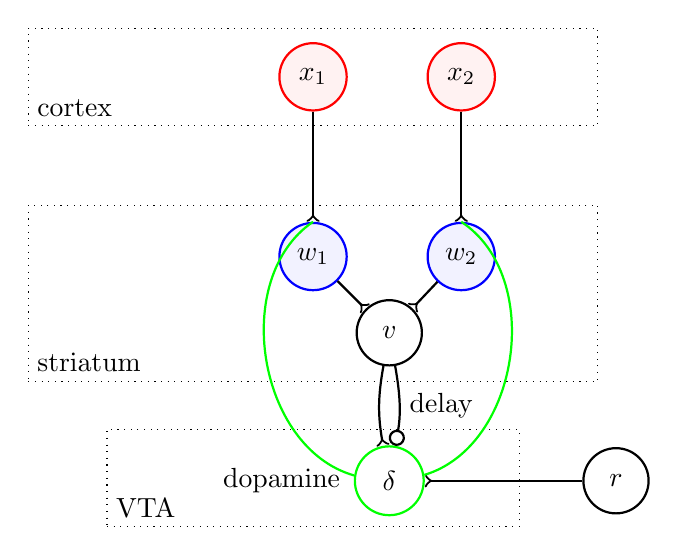
\begin{tikzpicture}
\node[text width=7cm, text height=1cm, draw=black, dotted](SC){cortex};
\node[align=center,text width=0.5cm,circle,draw=red, thick, fill=red!5](x1){$x_1$}; 
\node[align=center,text width=0.5cm,circle,draw=red, thick, fill=red!5, right = 1cm of x1](x2){$x_2$};
\node[text width=7cm, text height=2cm, draw=black, dotted,below =1cm of SC](St){striatum}; 
\node[align=center,text width=0.5cm,circle,draw=blue, thick, fill=blue!5,below = 1.4cm of x1](w1){$w_1$}; 
\node[align=center,text width=0.5cm,circle,draw=blue, thick, fill=blue!5, right = 1cm of w1](w2){$w_2$};
\node[align=center,text width=0.5cm,circle,draw=black, thick, below right= 0.5cm of w1](v){$v$};
\path (x1) edge[thick,-<] (w1);
\path (x2) edge[thick,-<] (w2);
\path (w1) edge[thick,-<] (v);
\path (w2) edge[thick,-<] (v);
\node[text width=5cm, text height=1cm, draw=black, dotted,below =0.6cm of St](VTA){VTA}; 
\node[align=center,text width=0.5cm,circle,draw=green, thick, below = 1cm of v](delta){$\delta$};
\node[left = 0.05cm of delta](d){dopamine};
\path (v) edge[thick,-o,bend left =10]node[right]{delay} (delta);
\path (v) edge[thick,-<,bend right=10] (delta);
\node[align=center,text width=0.5cm,circle,draw=black, thick, right= 2cm of delta](r){$r$};
\path (r) edge[thick,-<] (delta);
\path (delta) edge[thick,green,bend left =  65] (w1.north);
\path (delta) edge[thick,green,bend right = 65] (w2.north);
\end{tikzpicture}
\end{center}
\caption{A schematic of the VTA reward circuit. The conditioned
  stimulus is presented and this is communicated via the cortex,
  neurons in the striatum adjust this to give the input $w_ix_i$ and
  these are added producing the estimated reward. This inhibits a
  dopaminergic neuron in VTA, this neuron also receives excitatory
  input corresponding to the actual reward, this difference is
  $\delta$ and $\delta$ is effects dopamine modulation $w_1$ and $w_2$
  effecting some version of the  Rescorla-Wagner rule.\label{fig:tdl}}
\end{figure}

\subsection*{The VTA and hippocampus}

Back in Fig.~\ref{fig:VTA} we saw that VTA also projects to the
hippocampus; we have previously examined memory in the hippocampus so
it is interesting to speculate what the role of this projection is. In
\cite{LismanGrace2005a} it is argued that there is a signal from VTA
to hippocampal in which dopamine is used to mark novel and salient
stimuli, prompting their encoding in memory. In this model a new
stimulus is tested in CA1 to see if it is already stored in
hippocampus, if it isn't, this is communicated to VTA where the local
activity will test how novel, salient or surprising this stimulus is,
this is a role akin to, but slightly different from the role described
above in classical conditioning. If it is novel, activity in the
dopaminergic neurons increased long term plastic changes in
hippocampus. Evidence for this is found in \cite{MorrisEtAl2003a}
where it is shown that blocking dopamine receptors in hippocampus
reduces learning.

\begin{figure}
\begin{center}
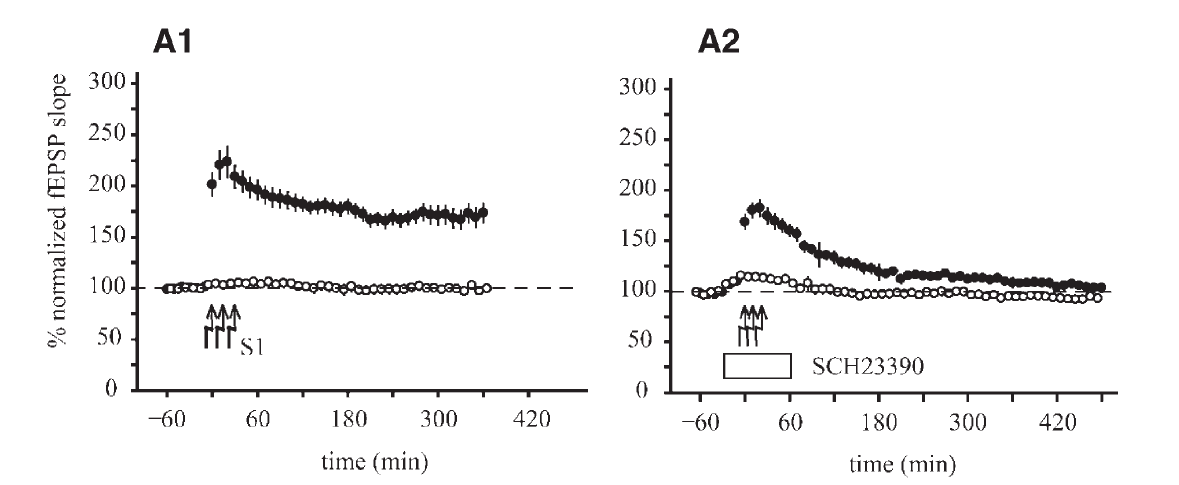
\includegraphics[width=10cm]{dopamine_learning.png}
\end{center}
\caption{In \textbf{A1} the change in strength of EPSPs is shown
  plotted against time, the synapse with closed circles has been
  stimulated to induce long term potentiation, the one with open
  circles is a control. In \textbf{A2} the same thing is done, but
  with dopamine receptors blocked during the stimulation. [Picture
    from \cite{LismanGrace2005a} which in turn adapted it from
    \cite{MorrisEtAl2003a}]\label{fig:hippocampus}}
\end{figure}



\begin{thebibliography}{10}

\bibitem{RescorlaWagner1972a}
Rescorla RA and Wagner AR. (1972) A theory of Pavlovian conditioning: Variations in the effectiveness of reinforcement and nonreinforcement, 
\newblock Classical Conditioning II, Black, AH and Prokasy WF, Eds., 64--99. Appleton-Century-Crofts.

\bibitem{DayanAbbott2001a}
Dayan P and Abbott FA. (2001) Theoretical neuroscience. 
\newblock  MIT press (Cambridge, MA).

\bibitem{MillerEtAl1995a}
Miller RR, Barnet RC and Grahame NJ. (1995) Assessment of the Rescorla-Wagner model.
\newblock Psychological bulletin 117: 363-86

\bibitem{AzorlosaCicala1986a}
Azorlosa JL and Cicala GA. (1986) Blocking of conditioned suppression with 1 or 10 compound trials.
\newblock Animal Learning and Behavior 14: 163--7.

\bibitem{SchultzDayanMontague1997a}
Schultz W, Dayan P and Montague PR. (1997) A neural substrate of prediction and reward.
\newblock Science 275: 1593--9.

\bibitem{Sutton1988a}
Sutton R (1988) Learning to predict by the methods of temporal differences.
\newblock Machine Learning 3: 9--44.

\bibitem{SuttonBarto1998a}
Sutton R and Barto S (1998). Reinforcement Learning.
\newblock MIT Press (Cambridge, MA).

\bibitem{Barto1995a}
Barto AG. (1995) Adaptive critics and the basal ganglia.
\newblock Models of information processing in the basal ganglia. Eds.
Houk JC, Davis JL and Beiser DG. MIT press (Cambridge, MA).

\bibitem{LismanGrace2005a}
Lisman JE and Grace AA (2005) The hippocampal-VTA loop: controlling the entry of information into long-term memory.
\newblock Neuron 46: 703--13.

\bibitem{MorrisEtAl2003a}
Morris RG, Moser EI, Riedel G, Martin SJ, Sandin J, Day M and O’Carroll C (2003) Elements of a neurobiological theory
of the hippocampus: the role of activity-dependent synaptic plasticity in memory. 
\newblock Philosophical Transactions of the Royal Society. 358: 773--786.

\end{thebibliography}

\end{document}
